% !TEX root = ../Thesis.tex
\chapter{Background}

%This is the body of the thesis.

%\section{Section}
%\label{sec:mylabel}

%\subsection{Sub-Section}

%\subsubsection{Sub-Sub-Section}

%\paragraph{Paragraph}

%\subparagraph{Even Sub-Paragraph}

%Testt This is the body text. Make sure that when you reference anything you use labels and references. When you refer to anything, you normally capitalise the type of object you reference~\ref{sec:mylabel} to, e.g. Section~\ref{sec:mylabel} instead of section~\ref{sec:mylabel}. You may also just use the \texttt{cref} command and it will generate the label, e.g., for \cref{sec:mylabel}, we did not specify the word ``Section''.

%Hint: Try to structure your labels as it is done with \texttt{sec:my-label} and \texttt{fig:machine}, etc.

%A Turing Machine is a 7-Tuple:
%\begin{equation}
    %M = \langle Q, \Gamma, b, \Sigma, \delta, q_0, F \rangle
%\end{equation}
%A Turing Machine is a 7-Tuple even if defined in the text, as in $M = \langle Q, \Gamma, b, \Sigma, \delta, q_0, F \rangle$.

Important concepts that are used in this thesis are presented in this section. A Summary of LoRa Technology, a short description of the Pycom devices and an overview of the TinySSB Protocol and its functionality follow.
\section{Long Range (LoRa) Wireless Technology}
\label{sec:lora}
In recent years the number of devices connected to the Internet of Things (IoT) has been increasing rapidly. Since a lot of those devices do not need to transfer high amounts of data and rather focus on using as little energy as possible, LoRa and similar technologies have been developed to serve those use-cases. In this section we will give a short overview of how LoRa works and how we can adjust its parameters. \\
LoRa promises long battery life, far-reaching communication distances (10 to 15 kilometres if devices are in line-of-sight) and high node density (nodes in close proximity can operate at the same time if configured correctly). The downside of having all those practical features is a lower data rate. To achieve this, it uses chirp spread spectrum modulation. Data that has to be sent is converted into \textit{upchirps} and \textit{downchirps}. Chirping up or down refers to a signal that is sent with constantly increasing or decreasing frequency. To adjust the transmission settings optimally to specific environments, different parameters that alter the chirps can be configured individually. One of those parameter is the \textbf{bandwidth}. The bandwidth is the difference in frequency of the start and end of one chirp and is typically set to 125, 250 or 500kHz. A higher bandwidth increases the acceptable transmission distance. Another parameter is the \textbf{spreading factor}. It determines the angle of one chirp. The higher the spreading factor, the longer it takes to complete one chirp. This can increase the transmission distance but reduces the data rate. Additionally to the physical settings we can set different \textbf{coding rates} which determine the forward error correction. A higher coding rate leads to a more reliable reception of packets and a lower data rate.
For our project we use a spreading factor of 7, bandwidth of 250kHz and a coding rate of 4/7. These settings have worked well to test the software but need to be reconsidered once the devices get deployed depending on the surrounding conditions.
\begin{figure}
\centering
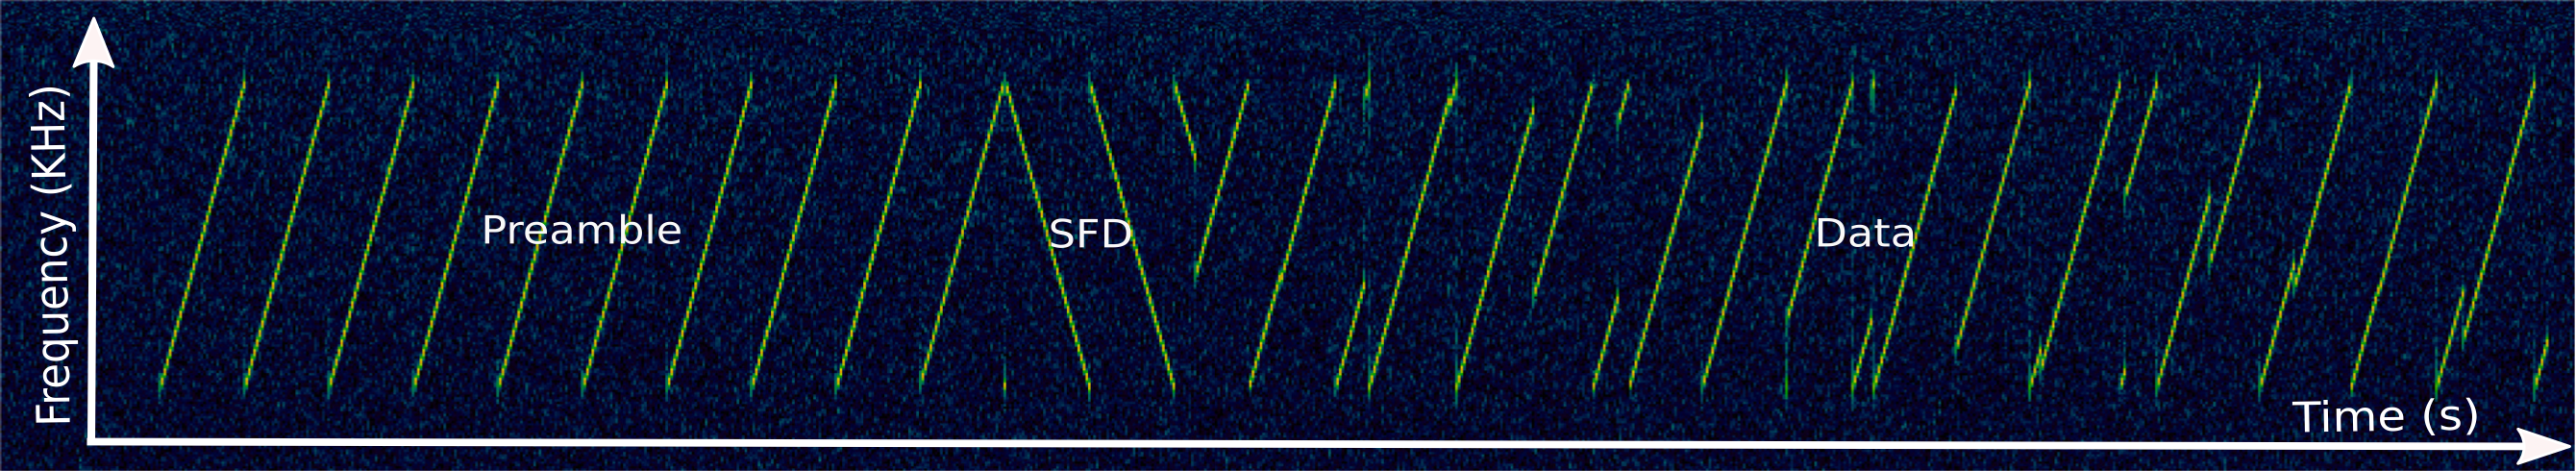
\includegraphics[width=1\textwidth]{chirps}
\caption{A visualized lora packet transmission. Source:~\cite{10.1145/3293534}}
\label{fig:chirps}
\end{figure} \\
In \cref{fig:chirps} we can see ten upchirps (preamble) and two downchirps (start frame delimiter) followed by modulated chirps that contain the actual data. 

(Sources for \cref{sec:lora} are~\cite{10.1007/978-3-030-01168-0_11} and~\cite{10.1145/3293534})

\section{Overview of TinySSB}
\subsection{Pure25519 Signature and Hash functions}
Two very important concepts in TinySSB that are used at various different points in the system are signature and hash functions. The importance of signatures will be discussed in \cref{sec:signing}. The algorithm that is used in this thesis is the ed25519 elliptic curve. [ADD SOURCE] It is used in TinySSB to digitally sign packets on one device and verify the signature on another device. To be able to achieve this, a key-pair has to be created first. The key-pair consists of a public key and a secret key. The algorithm then takes as input any message (in bytes) and the secret key that was created in the first step. The output is a digital signature. If any individual has access to the original message, the signature and the public key, they can verify the signature and confirm that the message was signed with the secret key that belongs to the public key used for verifying. \\
A hashing algorithm is used to convert a byte message with arbitrary length into a fixed size byte value. It is a deterministic algorithm, meaning that for any input, the algorithm will produce the exact same result every time. Additionally a person that knows the hash algorithm used and the resulting hash is not able to reconstruct the original input message. 
[CONTINUE HERE]
In TinySSB the sha256 hash algorithm is used. It takes any byte value as input and returns a 256 bytes value. 

\subsection{Signing and Verifying Packets}
\label{sec:signing}
TinySSB (Tiny Secure Scuttlebutt) is a protocol that is heavily influenced by SSB (Secure Scuttlebutt). An important concept of both protocols is the use of 'append-only-logs' or 'feeds'. In TinySSB a feed consists of a 128 byte feed header block containing some general information about the feed and any number of 128 bytes log-entries appended after it. Every node has one ID feed to be identifiable and an arbitrary amount of child and continuation feeds. [ADD REF]
\begin{figure}
\centering
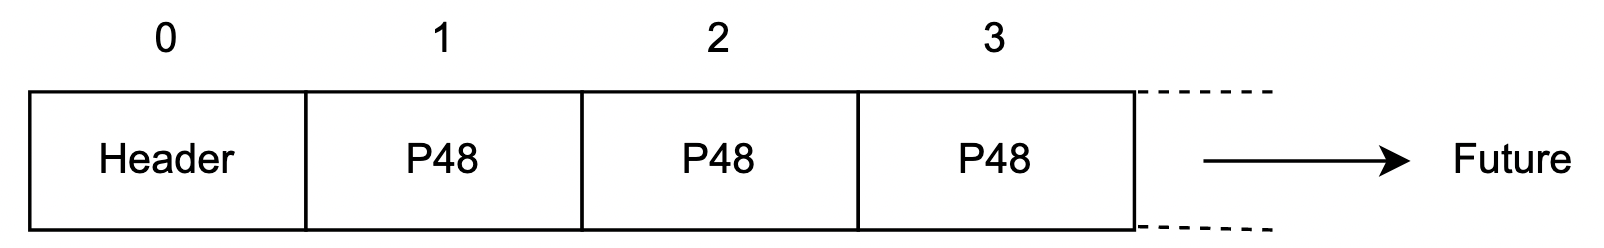
\includegraphics[width=1\textwidth]{feed}
\caption{Feed with the header block and three appended log entries. (P48 describes the standard packet type with 48 bytes payload)}
\label{fig:feed}
\end{figure}

To create a feed, a key-pair has to be calculated first. This is done using ed25519 elliptic curve cryptography. [ADD SOURCE]A key-pair consists of a public key - which also serves as the name and identification of the feed (feed ID) - as well as a secret key. These two keys have the following essential property for the TinySSB feed scheme. If a message is cryptographically signed with the secret key, the signature can (only) be verified with the corresponding public key. Every packet that is created and appended to a feed has to be signed by the feed owner with his secret key. This ensures that other nodes in the network - which know the feed ID - are able to verify that a message was indeed signed by the feed owner.

In \cref{fig:packets} we see two packets with the signature appended at the end. The first 8 bytes are not used and reserved for encryption purposes that will be implemented at a later stage. The next 7 bytes are used for demultiplexing. [ADD REF] The next byte specifies the type of the packet and the remaining 48 bytes are interpreted differently depending on the packet type. [CHECK THIS!]Using the first 64 Bytes, the signature and the public key of the feed, any node in the network can verify that the signature was created with the secret key corresponding to the public key and therefore trust the packet.\\

\begin{figure}
\centering
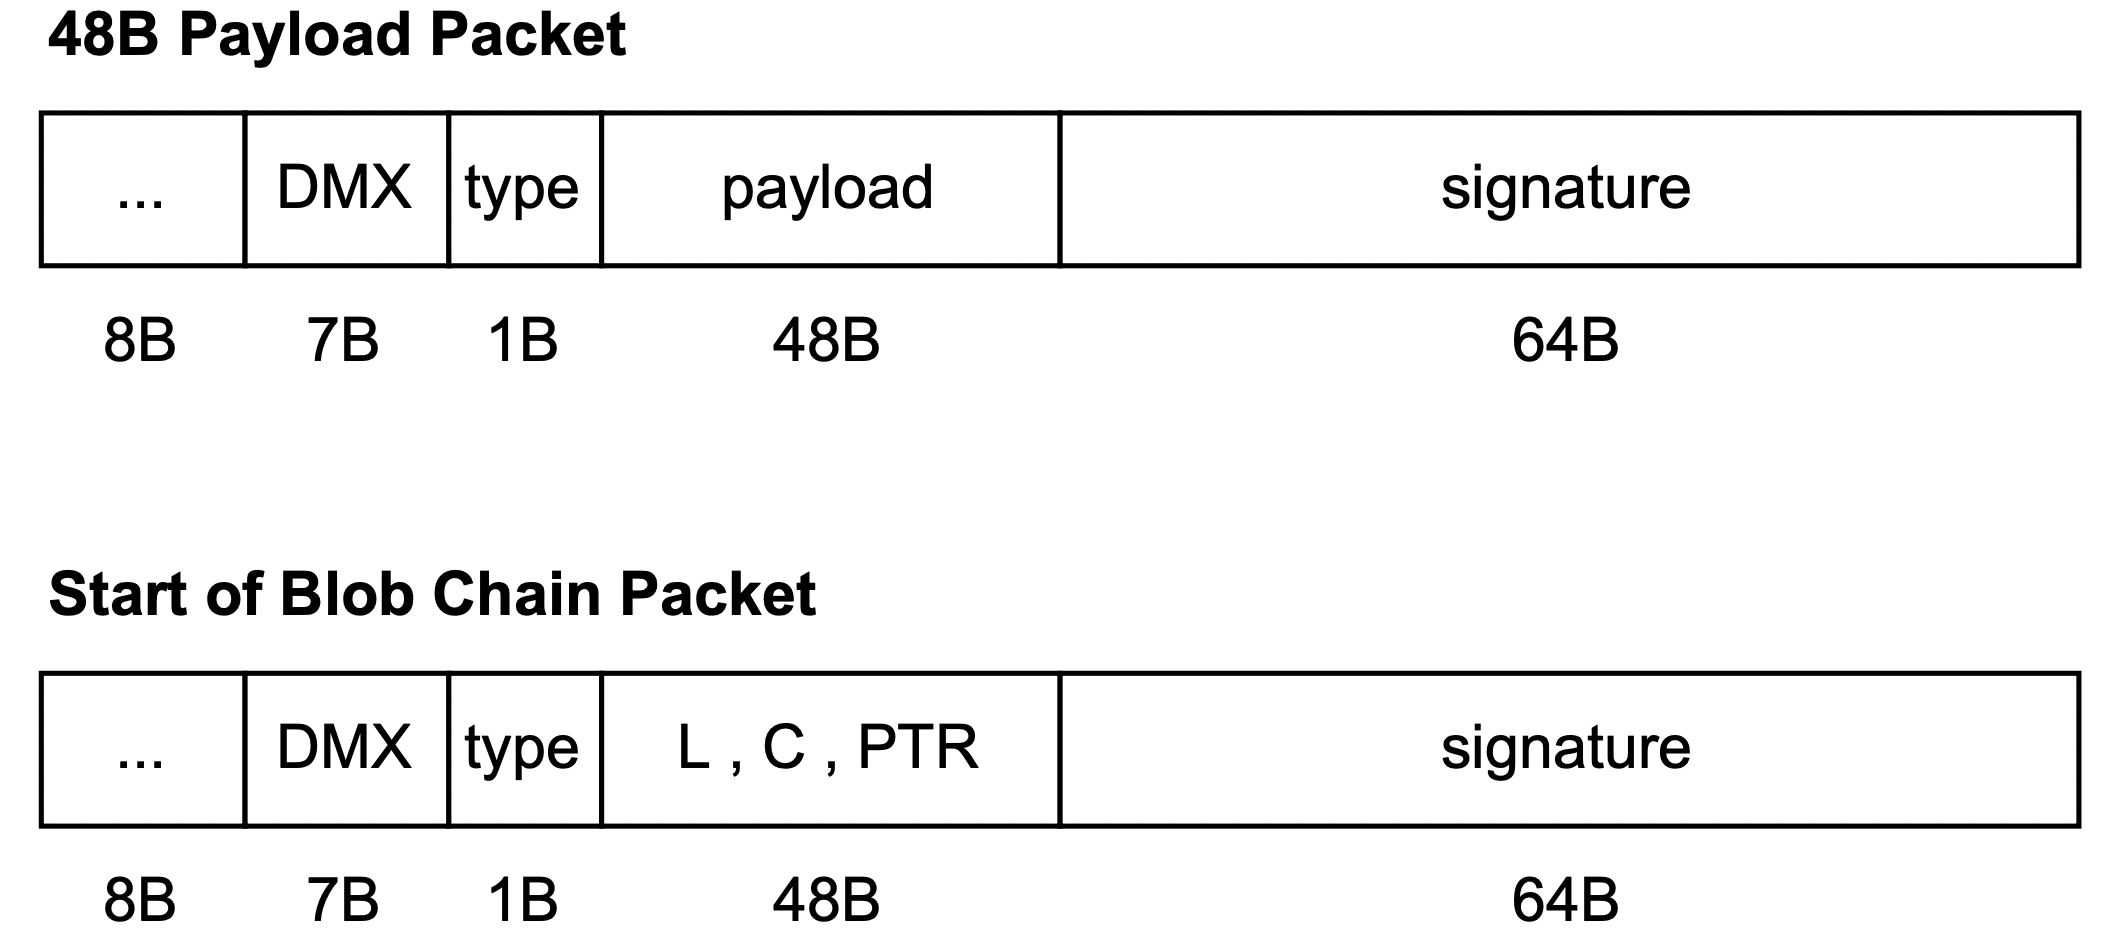
\includegraphics[width=0.9\textwidth]{packets}
\caption{Layout of two different packet types in TinySSB.}
\label{fig:packets}
\end{figure}

\subsection{Sending Data through the Network}
\label{sec:sending}
To propagate data through a TinySSB network, a receiving node has to replicate the feed of the sender. This means that if a feed gets transferred through a series of nodes, in the end every one of those nodes has a copy of the same feed stored on their device. (some replicas may be at a different state and have already more packets appended than others) As explained in \cref{sec:signing}, while replicating the feed, every node has to verify the signature of every packet starting at packet one up until the last packet in the feed. Suppose one node does not verify a malicious packet or intentionally appends a wrong packet to the feed, nodes that will receive those altered packets will not be able to verify them with the feed ID and therefore drop them immediately.

\begin{figure}
\centering
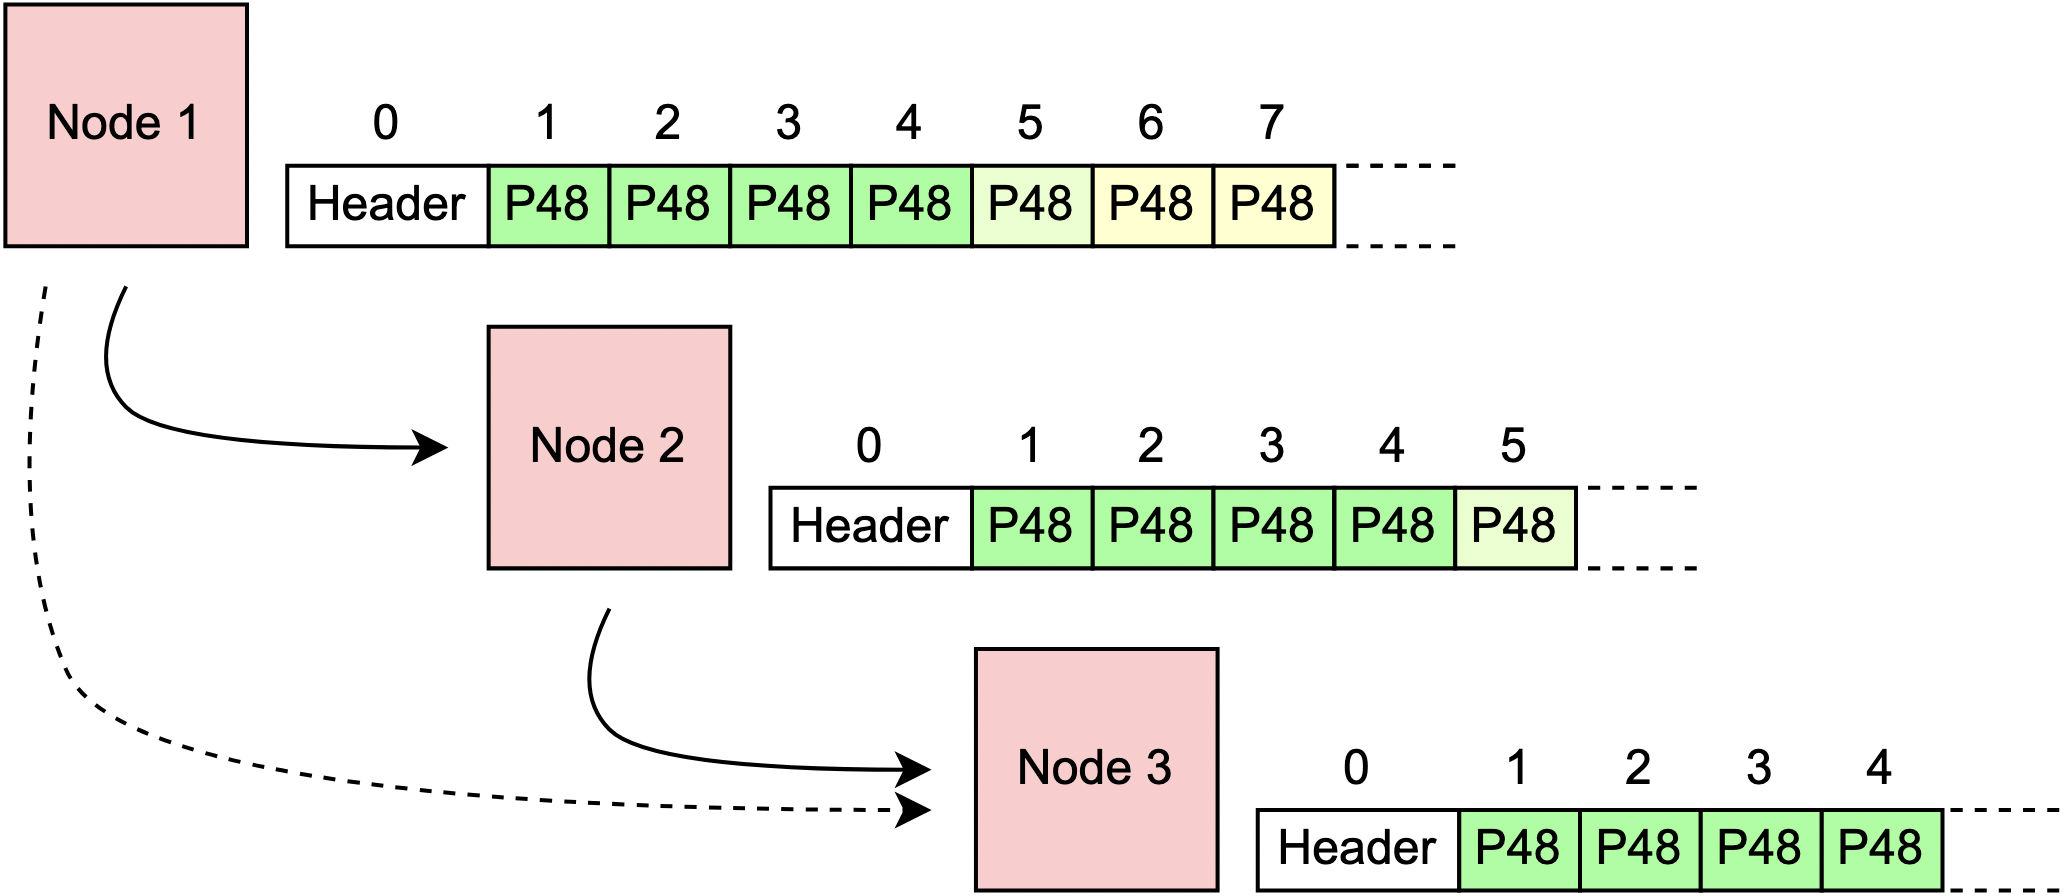
\includegraphics[width=1\textwidth]{replication}
\caption{The same feed forwarded over a series of three nodes. Node 1 is the feed owner and has already appended new packets that are not yet forwarded. Node 2 and 3 create their own replicas and try to catch up with Node 1. If Node 1 and 3 are geographically close enough, packets may even reach Node 3 directly from Node 1.}
\label{fig:replication}
\end{figure}

\subsection{Trust Anchors}
In \cref{sec:sending} we explored, how after successful verification nodes can append packets to feeds. Once a node has a replica of another feed, this is a straight forward process. However this does not yet explain how we can start a replication feed. If a node does not know the feed ID of a feed it wants to replicate, it cannot verify and trust its packets. To overcome this problem, we have to introduce \textbf{trust anchors}. Before a node can receive any packets from other nodes in the network, it has to be manually\footnote{At least one anchor has to be initialized manually. It would be possible to implement a higher authority / admin feed, that appends further anchors to its own feed and that way propagates anchors through the network.} initialized with trust anchors. A trust anchor refers to the feed ID of an identification feed of a node. If a trust anchor is installed, the node has the ability to verifying packets of the corresponding feed and start replicating it. While the first packet of a feed is directly dependent on the trust anchor to verify the signature, all the following packets can only be verified if a hash value of the previous packet is available. Since we have already established that we trust the previous packet, we can for that reason also trust the next packet. With this technique a trust chain is built that guarantees authenticity\footnote{No third party can alter the message.} and integrity\footnote{The message can only have been created by the owner of the feed.}. [REF POC?]

\subsection{Requesting Packets}
An important concept in TinySSB is \textit{how} packets are propagated through the network. Since the whole system builds on append-only-logs, every received packet has to be appended to a log. As a result of this, every node knows which packets it is expecting, namely for every feed the packet that follows the currently newest packet. We can make use of this convenient property by creating a list containing a 7 bytes long demultiplexing value\footnote{DMX value is calculated using the previous log entry, the feed ID, sequence number and a TinySSB specific version prefix. [REF TO TINY PAPER]} for every expected packet. With the help of this list, nodes can efficiently handle incoming packets. If the DMX field of an incoming packet is not contained in the DMX list, it can immediately be dropped. If it appears in the list, we can directly try to verify and append it to the corresponding feed. Using this DMX list, it is not necessary to include the feed ID, the sequence number or a backlink to the previous message in the packet. This info is concisely represented in the DMX value and therefore the packet size can be reduced to a minimum. (As opposed to the SSB implementation where this data and some additional information fields are included in every message~\cite{10.1145/3357150.3357396}) \\
Contrary to what \cref{fig:replication} might imply on first glance, network nodes do not arbitrarily send packets and hope that some other node receives them. This would be a very inefficient method. Instead - because nodes know which packets they are expecting - nodes will request the packets with a 'want broadcast'. This broadcast contains the feed ID\footnote{Instead of the complete feed ID the reduced form sha256(feed ID + b'want')[:7] + seq is sent.} and the sequence number of the desired packet. If a node that has the requested packet stored on its device receives such a message, it will send back the specified packet. This scenario is visualized in \cref{fig:request}. If the want request is unsuccessful and no packet is returned, the node has to wait for a given amount of time before trying to request the same packet again. If multiple nodes have the requested packet, they all will return the packet but only the fastest returned answer will be accepted.

\begin{figure}
\centering
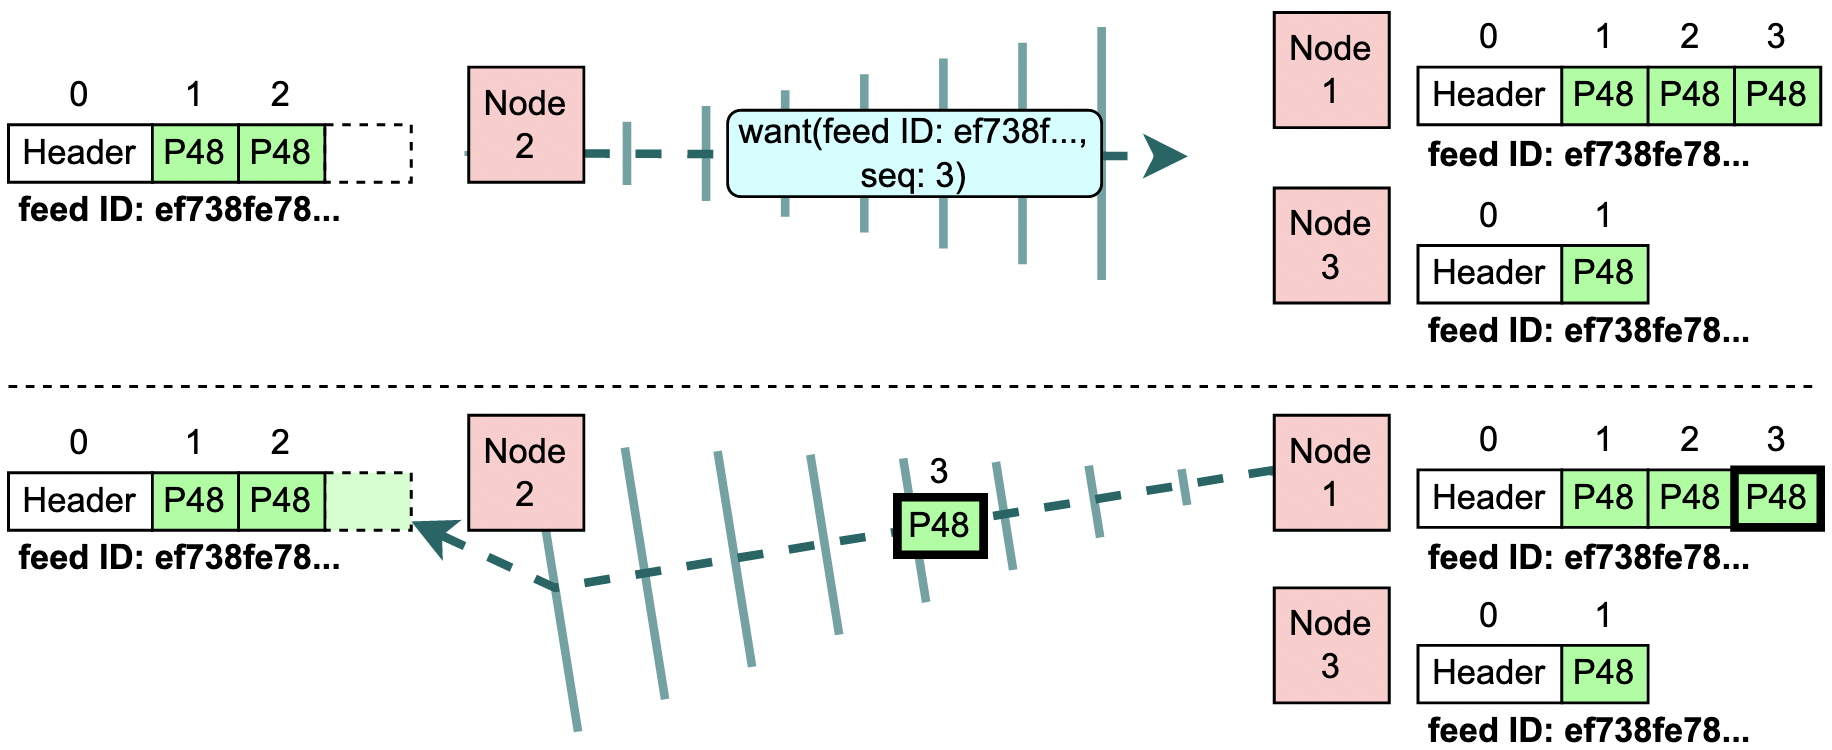
\includegraphics[width=1\textwidth]{request}
\caption{Node 2 requests packet with seq. nr. 3. Node 1 returns the requested packet. Node 3 does not have the requested packet and therefore does not answer.}
\label{fig:request}
\end{figure}

\subsection{Side Hash Chains}
When using 48 bytes payload packets, the size of data to be transferred is limited to 48 bytes or if larger has to be spilt up into chunks of 48 bytes with each chunk being divided among different consecutive packets. This would lead to a lot of overhead in terms of storage and network use. Therefore a more concise and efficient method is to use side hash chains. The data of a hash chain is (for the most part) not stored in a feed. It is stored in a separate folder in the file system in a file with size 120 bytes. Only the initial packet that points to the start of the chain is appended to the feed as a packet with type chain 20 (See second packet in \cref{fig:packets}). This packet - apart from the DMX, type and signature fields - contains the length of the hash chain, the first part of the payload and a hash pointer to the start of the chain. For chain packets, all fields that are typically used in standard packets can be omitted. Of the 120 bytes 100 are used for payload and 20 for the hash pointer to the next chain packet. A hash pointer is created by hashing the next chain packet. If the hash of the incoming chain packet matches the hash pointer of the previous packet, we can guarantee that the packet is the legitimate continuation of the chain. To be able to create such a chain, the sender must start by creating the last chain packet first and and appending its hash value to the second last packet. Then hashing the second last packet to append to the third last packet and so forth. This step has to be repeated backwards until the whole payload is split into hash chain packets before the first packet can be sent. A visualization of a sidehash chain is seen in \cref{fig:chain}. \\
\begin{figure}
\centering
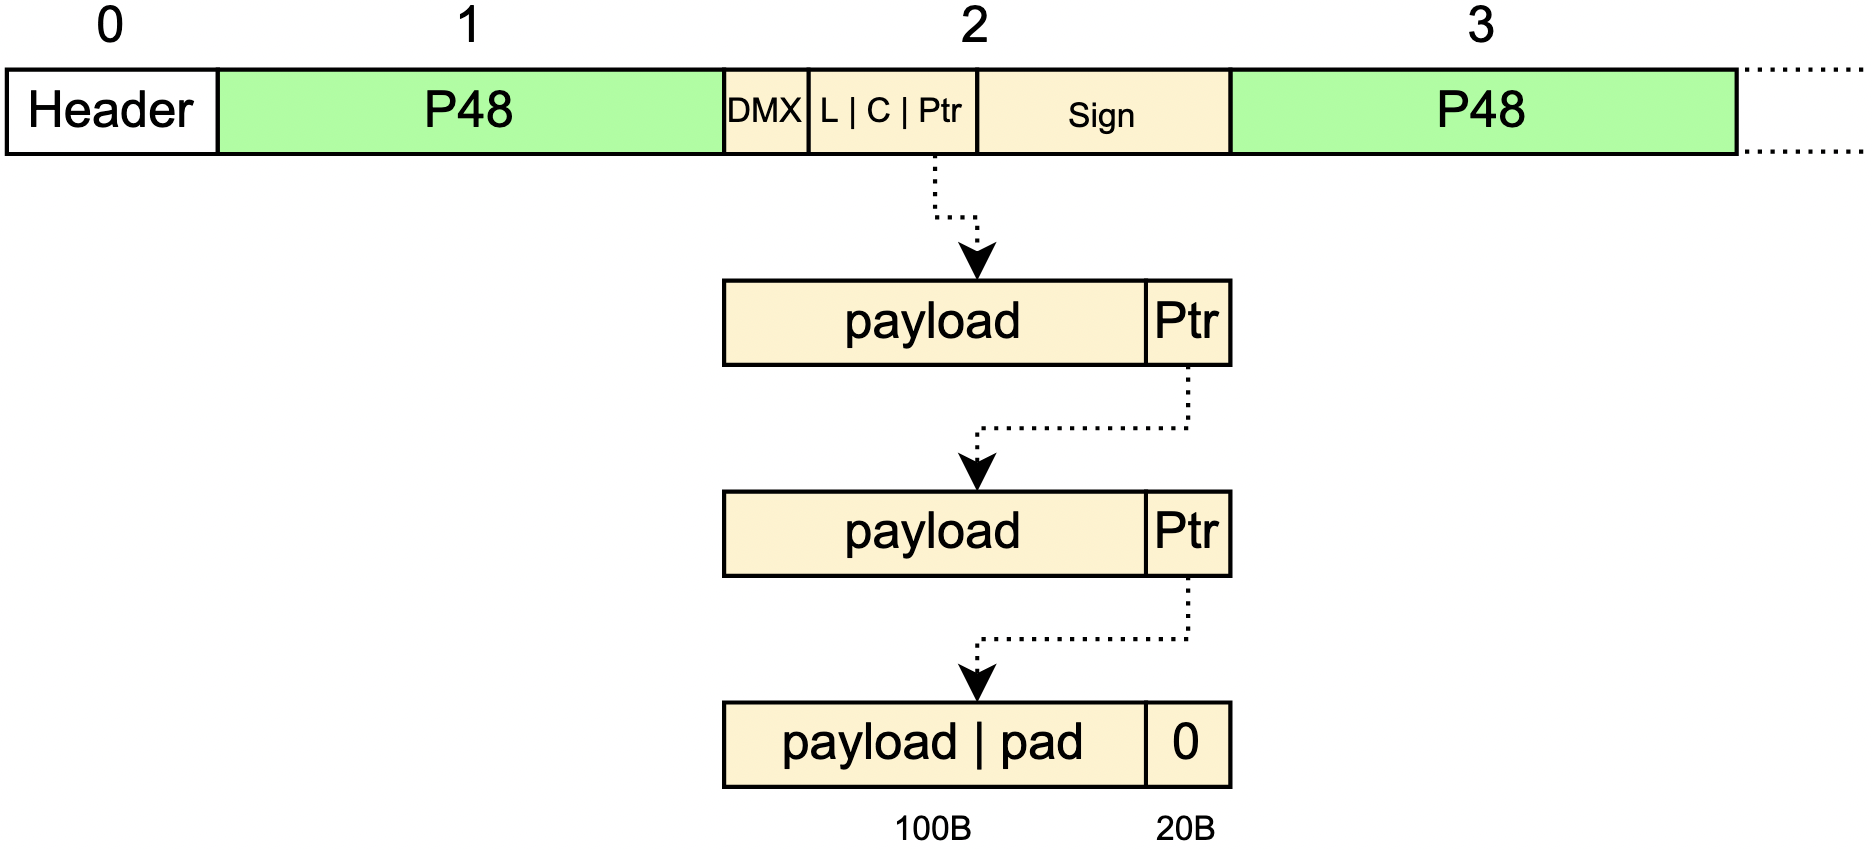
\includegraphics[width=1\textwidth]{chain}
\caption{Feed containing three packets. The second packet is of type chain 20 with a pointer to the next chain packet. In the last chain packet, the pointer is set to zero and a padding is added between the end of the payload and start of the pointer. Matching colors indicate a hash pointer to packet relation.}
\label{fig:chain}
\end{figure}

When a chain 20 packet is at the end of a feed, the whole chain has to be completely loaded before the next packet can be appended. The DMX table must therefore be updated by replacing the old DMX value with the hash pointer to the next chain packet. Thus if no matching DMX value could be found, the incoming packet has to be compared to the hash pointer values in the DMX table (in a second iteration). To request a chain packet, additionally to the feed id and sequence number the hash pointer has to be provided at the end of the want request. With those three parameters the correct chain packet can be found given that it is present on the device. \\


\subsection{Creating Child Feeds}
Considering that every node has only its one ID Feed where it appends all data, this one feed could quite rapidly become large, confusing and impractical. To tackle this problem we add more functionality to the append-only-log concept. We add two packet types that are used to create new feeds from within an existing feed. The first packet type declares a new child feed and the second packet type is used in the newly created feed to affirm it is a child feed.

\begin{figure}
\centering
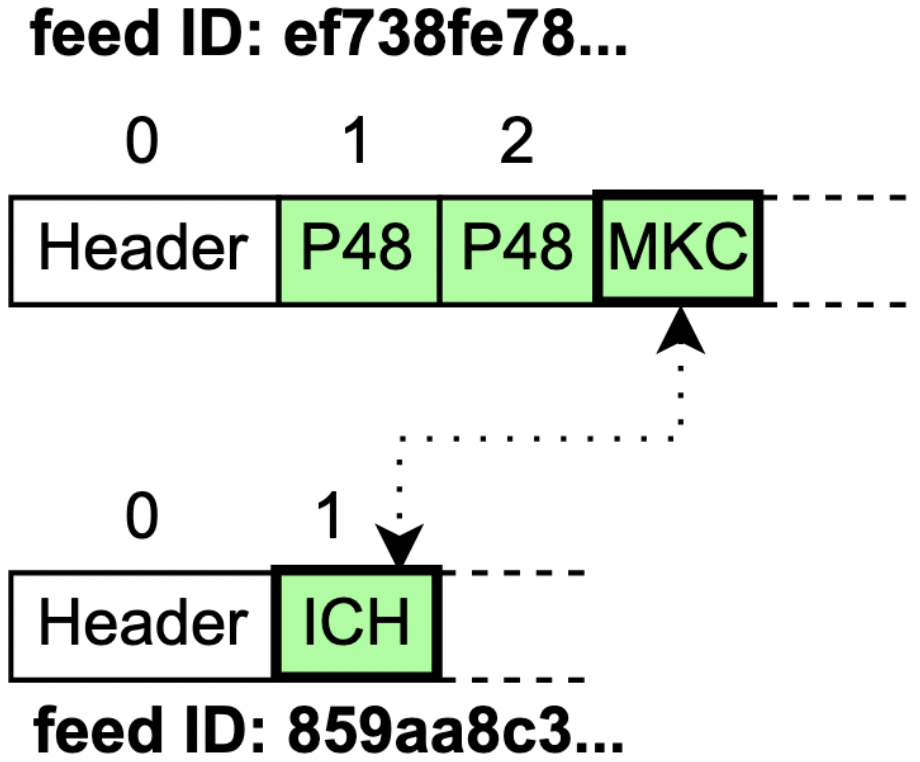
\includegraphics[width=0.4\textwidth]{mk_child}
\caption{The packet MKC declares a new child feed and points to the address 859aa... The packet ICH in the new feed indicates that it is a child feed and has an upward pointer to its parent feed.}
\label{fig:mk_child}
\end{figure}

The advantage of having multiple feeds is not only to separate packets for different applications into different feeds, it also has the practical advantage of now being able to request packets for both feeds individually. Depending on the importance of the feeds we can now optimize the request by prioritizing certain feeds over others. [ADD REF] Creating a child feed increments the number of entries in the DMX table which has to carefully manage the want requests to not overload the network or to use too much computing power. \\
The process of creating a new child feed is similar to creating the ID feed. First a new key-pair has to be created where the public key is used as the feed name and the secret key to sign packets. The node however now has to keep track of the new secret key as well. All key pairs that belong to the node's child feeds are stored in a config file and loaded into memory on start up. If the MKC (make child) packet reaches a node that replicates the feed, it will automatically create and replicate the child feed as well.

\subsection{Creating Continuation Feeds}
A feature with similar functionality is the creation of a continuation feed. The main idea behind this feature is to prevent feeds from becoming too long. There may exist feeds that get appended a lot of data and therefore grow at a rapid pace. When the feed gets bigger than a manageable size it becomes infeasible to propagate the whole feed through the network and store multiple copies of it on every device. For this use-case a packet type that declares a new feed as a continuation and a type that points to the previous feed are introduced.

\begin{figure}
\centering
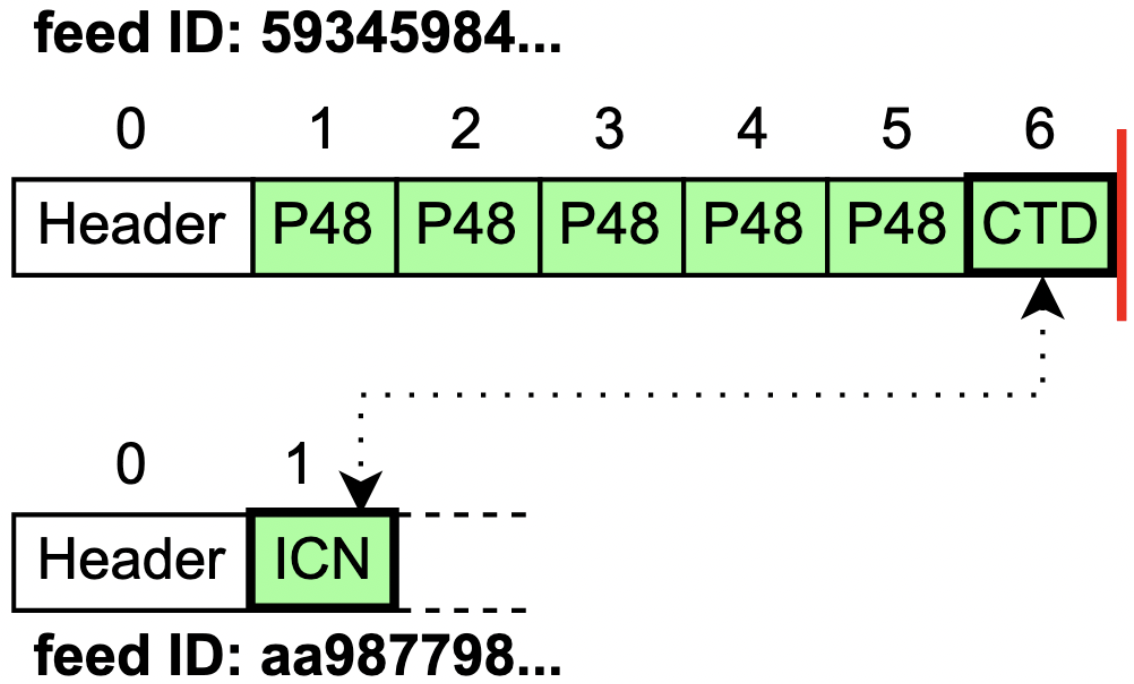
\includegraphics[width=0.5\textwidth]{mk_contd}
\caption{The packet CTD declares a new continuation feed and points to the address aa987... The packet ICN in the new feed indicates that it is a continuation feed and has a backward pointer to its previous feed. The red line indicates that no further packets can be appended.}
\label{fig:mk_contd}
\end{figure}

After a continuation packet is appended to a feed, log entries can no longer be appended, thus new packets for said feed do not need to be requested anymore. However the node still has to respond to incoming want request for the feed to be able to further propagate it through the network. The trust chain in this case is continued through the continuation packets. Using just continuation feeds as in \cref{fig:mk_contd} therefore does not free up storage space or come with any advantage, as still every node needs to build up the complete trust chain (now using two shorter separate instead of one longer feed). How continuation feeds can be useful will be discussed in [ADD REF TO SECTION]. As with child feeds, continuation feeds also have their own key-pairs that are stored in the same config file. If the address to the continuation feed is set to zero, this will be interpreted as ending the feed without continuation (No new feed will be created).

\subsection{Packet Types}

There are a number of different packet types in TinySSB, some of which were added on top while working on this thesis.
The first packet which can also be seen in \cref{fig:packets} describes a typical 48 bytes payload packet where the entire 48 bytes can be used for arbitrary data. The second packet seen in the same Figure is used to start a blob chain. 





%When a group of devices (network nodes) implement the TinySSB protocol, they can together form an independent network. All data that is sent and received over this network is stored in 'feeds'. Every network node needs to have its own key-pair consisting of a public and a secret key. Those two keys are mathematically related to each other and are later used to sign and verify messages. The secret key must be kept secret and not be distributed to other parties. The public key however can be propagated to other nodes. 

%In both protocols the creator of a message must be able to digitally sign messages while the receiver must be able to verify signatures. 



\section{Pycom 4}




%\section{Tables}
%Some tables can also be used as shown in \cref{tab:table}\footnote{Table captions are normally above the table.}. Remember that tables might be positioned elsewhere in the document. You can force positioning by putting a \texttt{ht!} in the definition.

%\begin{table}[ht!]
%\centering
%\caption{Frequency of Paper Citations. By the way: Make sure to put the label always after the caption, otherwise \LaTeX{} might reference wrongly!}
%\begin{tabular}{lcl} \toprule
%Title&$f$&Comments\\ \midrule
%The chemical basis of morphogenesis & 7327 & \\ 
%On computable numbers, with an application to the ... & 6347 & Turing Machine\\
%Computing machinery and intelligence & 6130 & \\ \bottomrule
%\end{tabular}
%\label{tab:table}
%\end{table}




%\section{Figures}
%Figures are nice to show concepts visually. For organising well your thesis, put all figures in the Figures folder. Figure~\ref{fig:machine} shows how to insert an image into your document. \Cref{fig:tm} references a figure with multiple sub-figures, whereas the sub-figures are referenced by \cref{fig:tm:tm1}, etc. \todoMissing{Description of figure.}

%\begin{figure}
%\centering
%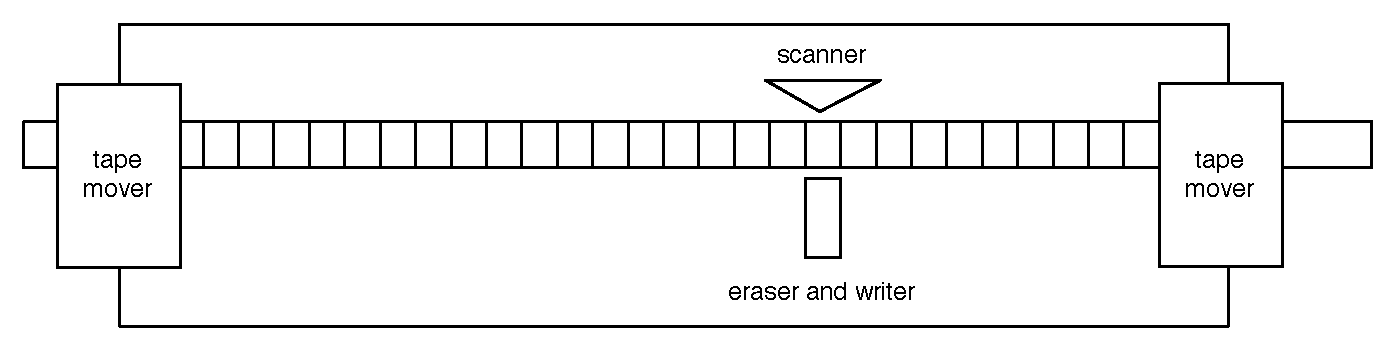
\includegraphics[width=0.9\textwidth]{turingmachine}
%\caption{A Turing machine.}
%\label{fig:machine}
%\end{figure}


%\begin{figure}
%\centering
%\subbottom[Turing Machine 1\label{fig:tm:tm1}]{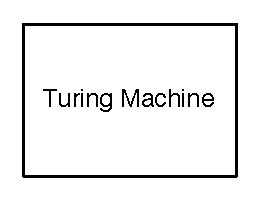
\includegraphics[width=0.2\textwidth]{block}}
%\subbottom[Turing Machine 2\label{fig:tm:tm2}]{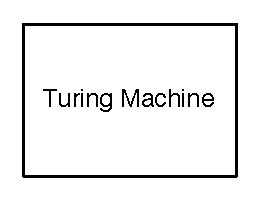
\includegraphics[width=0.2\textwidth]{block}}
%\subbottom[Turing Machine 3\label{fig:tm:tm3}]{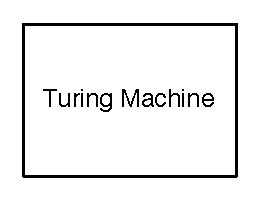
\includegraphics[width=0.2\textwidth]{block}}
%\subbottom[Turing Machine 4\label{fig:tm:tm4}]{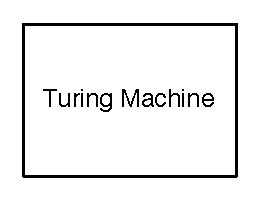
\includegraphics[width=0.2\textwidth]{block}}
%\caption{Plots of four Turing machines}
%\label{fig:tm}
%\end{figure}




%\section{Packages}
%These packages might be helpful for writing your thesis:

%\begin{description}
	%\item[\texttt{caption}] to adjust the look of your captions
	%\item[\texttt{glossaries}] for creating glossaries (also list of symbols)
	%\item[\texttt{makeidx}] for indexes and the back of your document
	%\item[\texttt{algorithm, algorithmicx, algpseudocode}] for adding algorithms to your document
%\end{description}